% ============================================================================
% 2000 年春季高考（京、皖）文科 第 14 题：三次函数 y = f(x) 的图象
% ----------------------------------------------------------------------------
% 来源：.work/phase4-b20/source/2000春季京皖文.pdf
%       SHA-256 b9552b8354735296f6ea1ed051085e094e4af0c14ff97ada2dbd4e579b14287f
%       第 1 页，内容流对象 39 / 40 / 42 / 43 / 44 / 45 / 46 / 47（按页面资源顺序拼接解析）
% 重绘方式：qpdf --qdf 取内容流 → 解析 m/l/c/re/S/f、w、d → 本地坐标
%          本地坐标 = 页面坐标 − (608.528, 616.430)，原点取坐标轴交点 O；
%          1 单位 = 1 TeX pt；页面为 A3（1190.55 × 841.89 pt）。
% 元素计数：实线路径 3（x 轴、y 轴、函数曲线），填充箭头 2，虚线路径 0，标签 5（y, O, 1, 2, x）
% 线宽：轴 0.40 pt；曲线 0.80 pt（内容流 w=0.79701）；箭头填充三角形长 3.99 pt、半宽 1.49 pt
% 坐标基准与源位的偏差：端点四舍五入到 0.001 pt；曲线按 299 段三次 Bézier 采样的折线重绘，经 0.02 pt 容差简化（57 点），最大偏差 < 0.02 pt。
% 标签：位置 = pdftotext -bbox 文本中心 − 基准；O 源位 (−7.998,−8.250)，左移 3.0 pt；1、2 源位 (17.012,−7.840)/(34.012,−7.840)，同步下移 2.4 pt；x 源位 (51.022,−5.590)，下移 1.8 pt；y 未动。净距均 ≥ 2 pt
% ============================================================================
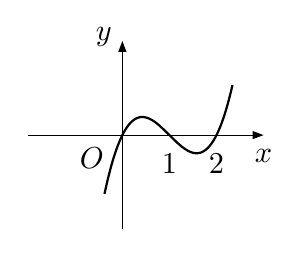
\begin{tikzpicture}[x=1pt, y=1pt,
    every node/.style={inner sep=0pt, font=\fontsize{10.5pt}{12.6pt}\selectfont}]
  % --- 坐标轴（轴身止于箭头底边，箭头为内容流中的独立填充三角形）
  \draw[line width=0.4pt] (-34.017,0) -- (47.438,0); % x 轴轴身
  \fill (51.025,0) -- (47.040,1.494) -- (47.040,-1.494) -- cycle; % x 箭头
  \draw[line width=0.4pt] (0,-34.017) -- (0,30.430); % y 轴轴身
  \fill (0,34.016) -- (1.494,30.031) -- (-1.494,30.031) -- cycle; % y 箭头
  % --- 三次函数曲线（内容流 299 段三次 Bézier → 0.02pt 容差 57 点折线）
  \draw[line width=0.8pt]
      (-6.463,-21.227) -- (-5.299,-16.066) -- (-4.112,-11.446) -- (-3.514,-9.357) -- (-2.894,-7.348) -- (-2.273,-5.498) --
      (-1.641,-3.772) -- (-1.020,-2.227) -- (-0.387,-0.801) -- (0.274,0.534) -- (0.936,1.721) -- (1.596,2.756) --
      (2.264,3.664) -- (2.954,4.458) -- (3.648,5.117) -- (4.364,5.656) -- (5.085,6.064) -- (5.809,6.343) --
      (6.573,6.507) -- (7.349,6.544) -- (8.125,6.460) -- (8.938,6.253) -- (9.783,5.921) -- (10.572,5.514) --
      (11.396,5.001) -- (12.266,4.374) -- (13.197,3.620) -- (15.059,1.923) -- (18.487,-1.468) -- (19.931,-2.837) --
      (21.408,-4.106) -- (22.104,-4.638) -- (22.791,-5.114) -- (23.581,-5.591) -- (24.343,-5.971) -- (25.065,-6.249) --
      (25.781,-6.439) -- (26.488,-6.535) -- (27.151,-6.536) -- (27.812,-6.445) -- (28.456,-6.262) -- (29.243,-5.904) --
      (30.019,-5.397) -- (30.784,-4.739) -- (31.549,-3.914) -- (32.286,-2.951) -- (33.006,-1.844) -- (33.721,-0.575) --
      (34.431,0.859) -- (35.118,2.422) -- (35.800,4.147) -- (36.490,6.077) -- (37.158,8.131) -- (37.817,10.340) --
      (38.494,12.801) -- (39.153,15.395) -- (39.785,18.071);
  % --- 标签
  \node at (-6.648,35.400) {$y$};
  \node at (-10.998,-8.250) {$O$};
  \node at (17.012,-10.240) {$1$};
  \node at (34.012,-10.240) {$2$};
  \node at (51.022,-7.390) {$x$};
\end{tikzpicture}
% ----------------------------------------------------------------------------
% 自验：轴端点 (−34.017,0)/(47.438,0) 与 (0,−34.017)/(0,30.430) 和内容流 574.5115/655.9662/582.4135/646.86 逐点吻合；曲线 57 点对源 Bézier 的最大偏差 < 0.02 pt；曲线与 x 轴交点 local x = −0.015 / 17.038 / 34.002，与标签 1、2 的横坐标 17.012 / 34.012 一致（偏差 < 0.03 pt）。标签净距（字形墨迹包围盒对路径中心线，已扣除线宽半宽）：y 3.30、O 2.14、1 4.00、2 2.41、x 2.95 pt，均 ≥ 2 pt。探针编译：xelatex 0 错误、0 警告。
% ============================================================================
